\begin{figure}[!t]
\centering
\tikzset{
every tree node/.style={align=center,anchor=north}
edge from parent/.style={very thick},
%edge from parent/.style=
%{draw, edge from parent path={(\tikzparentnode.south)
%-- +(0,-8pt)
%-| (\tikzchildnode)}},
blank/.style={draw=none}}
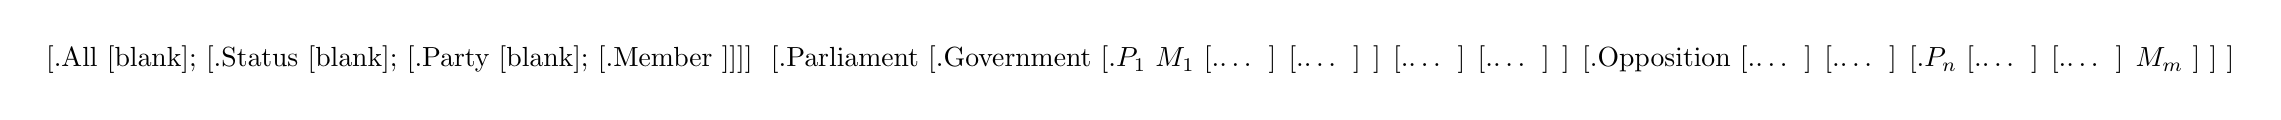
\begin{tikzpicture}[level distance = 30pt]
% \fontsize{7}{8}\selectfont
\matrix
{
\node{\Tree
    [.All  \edge[blank]; 
    [.Status  \edge[blank];
    [.Party \edge[blank]; 
    [.Member ]]]]};
&
\node{\Tree 
    [.Parliament
        [.Government
            [.$P_1$  $M_1$ [.{\dots} ] [.{\dots} ] ]
            [.{\dots} ]
            [.{\dots} ]
%            [.$P_n$  $M_1$ [.{\dots} ] $M_n$ ]
        ]
        [.Opposition 
%            [.$P_1$  $M_1$ [.{\dots} ]  $M_m$ ]
            [.{\dots} ]
            [.{\dots} ]
            [.$P_n$  [.{\dots} ] [.{\dots} ] $M_m$ ]
        ]
    ]};\\
};
\shrink
\end{tikzpicture}
\caption{\label{fig:ParHierarchy}Hierarchical relations in parliament.}
\end{figure}